\section*{Implementation}

\subsection*{Previous Setup}

Before the start of the project, small scripts were written in C++ and Python to visualize the molecular data. There was a separate Python script which performed the extraction of the data from the XML and a separate C++ script which computed the radial distribution function. After the two scripts were ran, the user then had to use the GNU plot to graph the respective outputs. The overall setup can be described by the three blocks in the picture:





With respect to the picture, the following files performed the following functions: 

\begin{itemize}
        
    \item \verb|qbox_xyz.py|: Progressively parses the given XML document and only scrapes the appropriate values defined in the \verb|sax_handler.py|. Handles the input data which is in a XML format which contain details about the simulation and outputs a .xyz simulation format to be used by the \verb|gofr.C| program.
    
    \item \verb|sax_handler.py|: This script stores the important data attributes required to scrape from the xml to used for the radial distribution computation and visualization in the later phases.

    \item \verb|gofr.C|: Performes the radial distribution algorithm to generate the density and probability functions based on the given atomset.
    
    \item \verb|unitcell.C|: Represented an abstraction of a cell which has x, y, and z coordinates in three dimensional space.
    
    \item \verb|./plotgofr|: A linux executable script which visualizes the final output data using GNU Plot.
    
\end{itemize}





One advantage of this approach was that the computation of the radial distribution function was very efficient. However, there were multiple problems with this approach:

\begin{itemize}
    \item Flexibility: This approach was not very flexible because a separate script had to be run during each phase of the process. In addition, the output data format was very similar to that of the GNU Plotting format, so if the user wanted to perform graphical analysis using a different software, it was a challenge.
    
    \item Usability: Since all these scripts used different languages and in some cases were platform dependent, integration was virtually absent. In other words, there was not one single platform which the user could run all the scripts but rather everything was split across different platforms and languages. In addition, the user had to switch between python, C++, and bash scripts which could be inconvenient in some cases. 
    
    \item Interactivity: This was probably the biggest problem with the previous approach. The generation of the graphs was static in the sense that if the user wanted to visualize atomsets of various sizes, he or she would need to run the corresponding scripts again and again for different configurations. In other words, there was not a way in which the user can \textit{interactively} examine and analyze the atomset data and visually examine how it would change over a period of time.
\end{itemize}

\subsection*{New Setup}

To eliminate most or all of the problems mentioned with the previous approach, a ``better'' solution was developed in terms of the scope of the project. Doing so involved developing and integrating all the scripts in one platform using one language. The main language of choice which was chosen during the development phase was Python. This was to make the scripts easier to run and also make code extremely portable and usable. However, one downside with this approach was the main performance of the radial distribution function. This was the only bottleneck in the pipeline. (The performance issues will be explained later sections). The overall pipeline of the following project was as follows:



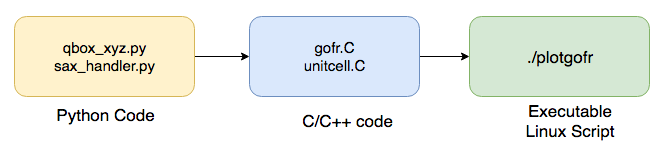
\includegraphics[scale=0.30]{images/old_pipeline}\newline


With respect to the new setup, the following files performed the following functions: 

\begin{itemize}
        
    \item \verb|qbox_xyz.py|: Mostly remains unchanged with respect to the previous setup.
    
    \item \verb|sax_handler.py|: Also mostly remains unchanged with respect to the previous setup.

    \item \verb|gofr.py|: Computes the radial distribution function and the probability density functions. This file represents the translation of the C++ gofr.C code to python code. 
    
    \item \verb|unitcell.py|: Represents an abstraction of a three-dimensional cell, however the main code is written in Python.
    
    \item \verb|run_gofr.py|: Runs the main gofr.py with the given inputs.

    \item \verb|visualizer.py|: This is an important file which generates a .html page containing the interactive visualization of the atomset.
    
\end{itemize}



\subsection*{Transition from C++ code to Python code}


\textbf{Differences}
Even though most of the functionality can be replicated and translated well in Python from C++, there are a few distinctions to be made. For instance, the operator overloading feature in C++ is a common practice whereas higher level languages such as Python or Java use function calls to replicate the effect. This was indeed the case with files such as \verb|unitcell.py|. In the C++ code, operators such as / (division), * (multiplication), etc were overloaded for vectors whereas the Python code achieved the same effect using function calls such as \verb|scalarProduct()| , \verb|length()|, etc.

Some other difference with the Python code was making the scripts as modular as possible in order to debug and create an efficient and a clean pipeline. Doing so not only improves code readability but is also easy to maintain. 

\textbf{Similarities}

The C++ code and Python code have a lot of similarities, especially for files such as \verb|UnitCell| and |gofr|. The code and logic were mostly translated line by line from C++ and Python, and therefore the name of function calls and the constructors have also been provided the same names. The Object-Oriented paradigm has also been preserved across the translation and therefore the \verb|UnitCell.py| and \verb|Gofr.py| have corresponding constructors along with getters and setters. 

\subsection*{Performance Issues during translation}

The biggest challenge encountered was the performance of the radial distribution algorithm in Python. In short, this algorithm has a $O(n^2)$ time complexity.  

\begin{lstlisting}[language=Python, caption=Python Code which computes the gofr.]
 for i in range(species_1_count):
    for j in range(species_2_count):
      first_vector = tau[isp1[i]]
      second_vector = tau[isp2[j]]
      
      difference_vector = [ai - bi for ai, bi in zip(first_vector, second_vector)]
      difference_vector = uc.fold_in_ws(difference_vector)
      scaled_vec = [x / dr for x in difference_vector]
      
      length_scaled_vec = sqrt(scaled_vec[0] ** 2 + scaled_vec[1] ** 2 + scaled_vec[2] ** 2)
     
      k = (int) (length_scaled_vec + 0.5)
      if k < nbin:
        count[k] += 1
\end{lstlisting}

In terms of functionalities, both pieces of code produce the same results, however they vary significantly in performance. For instance, running the C++ code on $2,000$ atomsets takes about $50$ seconds, whereas when the same corresponding Python code takes $15$ mins! This is due to the nature of the interpreted languages and restrictions to manipulations at lower levels. In addition, the C++ code can be precompiled with some optimizations depending on the platform, which yields efficient results. In summary, the differences in performance can be highlighted in the following table:

\begin{center}
\begin{tabular}{ |c|c|c| } 
 Size of Atomset & Performance time in Python & Performance time in C++ 
 \hline
 $20$ & $5$ sec & $9$ sec \\ 
 $2000$ & $50$ sec & $15$ \textit{mins} \\ 
 \hline
\end{tabular}
\end{center}


\subsection*{New Features Added during translation Phase}

\begin{itemize}

\item Stepsize: Several new features were added during the translation. For instance, the precomputed radial function values were stored for every $n^{th}$ stepsize. By doing so, the entire application was made customizable and interactive for the visualization phase. 

\item Visualization: This was a powerful addition to the entire application. The visualization was performed in javascript and a corresponding python script generated the html page. In addition, the visualization was interactive and customizable according to the user's needs.

\end{itemize}

\subsection*{Customizability according to user's needs}

To customizable according to the user's needs, the application has a configuration file. In this file, there are various parameters which the user can adjust according based on the goal of interest. The configuration file looks like the following:

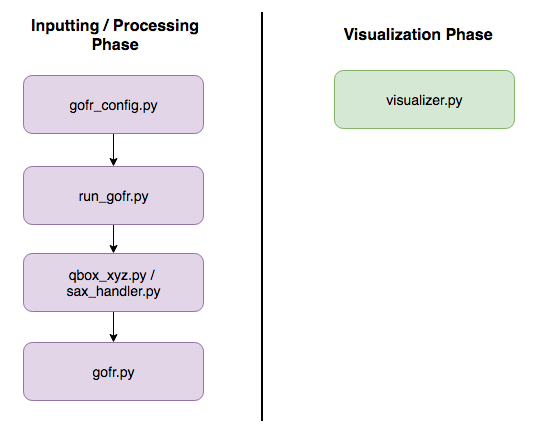
\includegraphics[scale=0.30]{images/new_pipeline}\newline

\begin{lstlisting}[language=Python, caption=Config file for setting parameters during the run.]
# Configuration file

first_input_source = "./input_files/md120_short.r"
second_input_source = './input_files/md120_short2.r'
all_or_first = "a"

first_molecule_name = "H"
second_molecule_name = "H"
rmax = 5
dr = 0.05
stepsize = 1
\end{lstlisting}


